\documentclass[a4paper,12pt]{article}

% --- Packages for better readability and layout ---
\usepackage[utf8]{inputenc}
\usepackage[T1]{fontenc}
\usepackage{lmodern}    % Better fonts
\usepackage[english]{babel} % Language settings
\usepackage[margin=1in]{geometry}
\usepackage{microtype}  % Microtypography
\usepackage{setspace}
\setstretch{1.1}

% --- Math, Graphics, and floats ---
\usepackage{amsmath}
\usepackage{graphicx}
\usepackage{float}      % Enables [H] option
\usepackage{caption}
\usepackage{subcaption} % For subfigures (optional)
\usepackage{booktabs}   % For better tables

% --- Hyperlinks ---
\usepackage{hyperref}
\hypersetup{
    colorlinks=true,
    linkcolor=blue,
    urlcolor=blue,
    pdftitle={Analysis Report},
    pdfpagemode=FullScreen,
}

\title{Trends in CO\textsubscript{2} Emissions and Temperature Variability in the Americas}
\author{Florian Merlau}
\date{\today}

\begin{document}
\maketitle

\section{Introduction}
Over the past few decades, CO\textsubscript{2} emissions in North and South America have changed considerably, often accompanied by rising regional temperatures. These developments are important for understanding environmental and socio-economic impacts. This report examines the temporal trends in CO\textsubscript{2} emissions and temperature variability across North and South America, with an emphasis on identifying principal contributors and assessing regional differences. The analysis uses two comprehensive datasets to explore the relationship between emissions and temperature changes, thereby providing insights into this significant aspect of climate science. 

\section{Used Data}
This project relies on two datasets from \textit{Our World in Data} that provide key insights into global climate change and CO\textsubscript{2} emissions.

\noindent
The first dataset records global monthly average surface temperatures, measured 2\,meters above ground across land, sea, and inland water surfaces. It includes yearly and monthly temperature values in degrees Celsius, highlighting seasonal variations and long-term trends, with a focus on recent anomalies. The data span from 1960 to the present and were sourced from Our World in Data:  
\url{https://ourworldindata.org/grapher/monthly-average-surface-temperatures-by-year}

\noindent
The second dataset tracks annual CO\textsubscript{2} emissions from fossil fuels and industrial processes between 1750 and 2023. Emissions are presented in metric tonnes by world regions, including major emitters such as China, the United States, and the European Union. International aviation and shipping emissions are reported separately. The data were also obtained from Our World in Data:  
\url{https://ourworldindata.org/grapher/annual-co-emissions-by-region}

\noindent
Both datasets are licensed under the \textit{Creative Commons BY license} and are appropriately cited to comply with licensing requirements. The temperature data are sourced from the Copernicus Climate Change Service (2019, 2025), while the emissions data come from the Global Carbon Budget (2024). These datasets form the foundation for analyzing the relationship between rising temperatures and CO\textsubscript{2} emissions, providing a comprehensive basis for the project.

\section{Methodology}
This study analyzes temperature changes and CO\textsubscript{2} emissions in North and South America through a structured pipeline of data retrieval, cleaning, transformation, and visualization. Relevant datasets, including annual emissions and monthly surface temperatures, were retrieved from online sources and cleaned by removing duplicates, handling missing values, and dropping irrelevant columns.

\noindent
The temperature data were transformed into an analyzable format by unpivoting and standardizing columns. Both datasets were filtered for common years and countries within two defined regions: North America (e.g., Canada, USA, Mexico) and South America (e.g., Brazil, Argentina, Chile). The datasets were merged based on shared attributes (e.g., year, region, country) to create a combined dataset of temperature and emissions.

\noindent
To simplify the analysis, data were grouped by year, calculating average temperatures and total emissions. Trends and relationships were visualized using linear and polynomial regression models, along with interactive plots, to highlight temporal changes and correlations between emissions and temperature.

% --- Abb. 1 ---
\begin{figure}[htbp]
    \centering
    \includegraphics[width=0.5\textwidth]{pics/tabelle.png} 
    \caption{Summary of the datasets utilized in the project.}
    \label{fig:dataset-overview}
\end{figure}

\section{Analysis Results}

\subsection{CO\textsubscript{2} Emissions in North America}
In North America, the United States is the primary source of CO\textsubscript{2} emissions, with levels rising steadily from 1950 and peaking in 2007 at over 6 billion metric tons. A subsequent decline is evident, reflecting the effects of energy efficiency improvements and the adoption of renewable energy. Canada and Mexico contribute considerably less to the region’s total emissions.

% --- Abb. 2 ---
\begin{figure}[htbp]
    \centering
    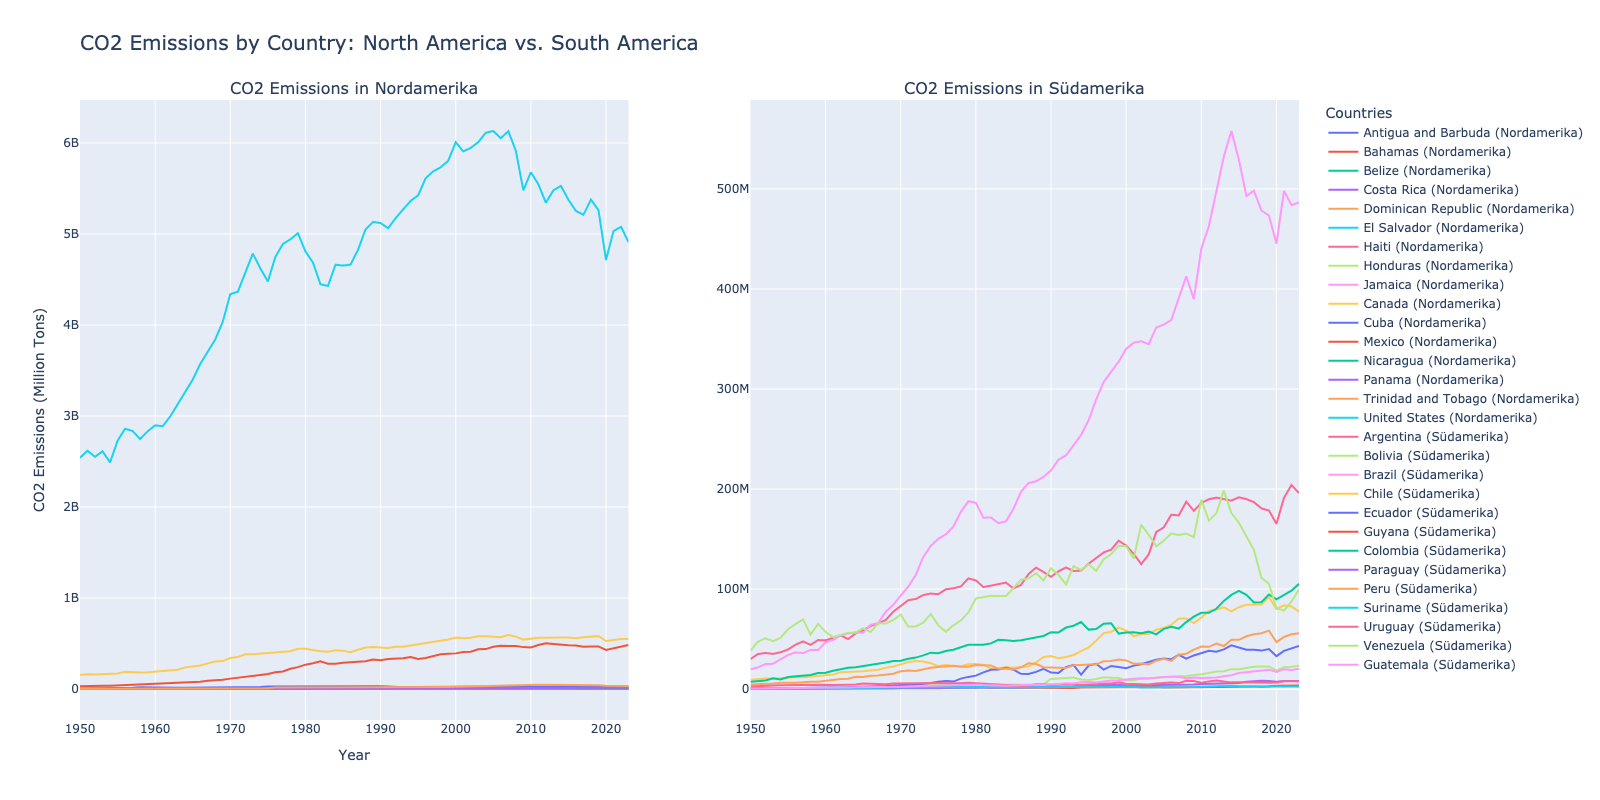
\includegraphics[width=\textwidth]{pics/co2_emissions_large_graph.png} 
    \caption{CO\textsubscript{2} emissions trends in North and South America.}
    \label{fig:co2-emissions}
\end{figure}

\subsection{CO\textsubscript{2} Emissions in South America}
In South America, emissions are significantly lower overall. Brazil emerges as the largest contributor, with steady growth attributed to industrialization and deforestation. Other countries, such as Argentina, Venezuela, and Colombia, display moderate increases, while smaller nations contribute negligibly (see Figure~\ref{fig:co2-emissions}).

\bigskip

\subsection{Temperature Trends}
The temperature trends in North America, depicted with a blue line and a red dashed regression line, show a slight upward trend. The regression line indicates a gradual increase in average temperatures over the observed period. Similarly, South America exhibits a positive trend in temperatures, shown by the green line and the purple dashed regression line. The slope of the South America regression line suggests a slightly faster increase in average temperatures compared to North America (see Figure~\ref{fig:regression-overview}).

% --- Abb. 4 ---
\begin{figure}[htbp]
    \centering
    \includegraphics[width=\textwidth]{pics/gesamt.png} 
    \caption{Overview of CO\textsubscript{2} emissions and temperature trends regression analysis.}
    \label{fig:regression-overview}
\end{figure}

\noindent
Both regions display consistent temperature fluctuations around the regression lines, but the increasing slopes highlight long-term warming trends.

\subsection{Correlation between Emissions and Temperature}
The scatter plot reveals distinct patterns for the two regions. In North America, a positive correlation between CO\textsubscript{2} emissions and temperature is evident. As emissions increase, temperatures tend to rise, albeit with variability. This pattern reflects the influence of industrial activity and energy consumption on regional warming (see Figure~\ref{fig:corr}).

% --- Abb. 5 ---
\begin{figure}[htbp]
    \centering
    \includegraphics[width=\textwidth]{pics/corr.png} 
    \caption{Correlation between CO\textsubscript{2} emissions and temperature in North and South America.}
    \label{fig:corr}
\end{figure}

\noindent
In South America, a similar positive correlation is observed, with temperatures rising as CO\textsubscript{2} emissions increase. However, the slope appears less steep compared to North America, which may be due to lower emissions levels and differing climatic or environmental factors (see Figure~\ref{fig:corr}).

% --- Abb. 3 ---
\begin{figure}[htbp]
    \centering
    \includegraphics[width=0.7\textwidth]{pics/p_value.png} 
    \caption{Statistical analysis of regression results.}
    \label{fig:regression-results}
\end{figure}

\noindent
For South America, the slope is \(1.58 \times 10^7\), which also indicates an upward trend in emissions, though at a slower rate compared to North America. The R-squared value of 0.9669 reflects a very strong model fit, explaining 96.69\% of the variance in emissions. The p-value (\(5.15 \times 10^{-55}\)) strongly supports the statistical significance of this trend.

\noindent
The regression results for North America show a positive slope of \(5.99 \times 10^7\), indicating a steady increase in CO\textsubscript{2} emissions over the analyzed period. The R-squared value of 0.8069 suggests that approximately 80.69\% of the variability in emissions can be explained by the model, indicating a good fit. The p-value (\(2.01 \times 10^{-27}\)) confirms the trend is statistically significant (see Figure~\ref{fig:regression-results}).


\section{Conclusion}

The analysis shows a clear link between rising CO\textsubscript{2} emissions and increasing temperatures in both North and South America. North America, led by the United States, has higher emissions and more pronounced warming trends, while South America exhibits slower but significant increases. These findings highlight the urgent need for emission reductions to mitigate climate impacts.

\end{document}
